\documentclass[tikz,border=0pt]{standalone}
\usepackage{amsmath, amssymb}
\usetikzlibrary{matrix, positioning, fit, backgrounds, calc}
\usepackage{helvet}
\usepackage{avant}
\renewcommand*\familydefault{\sfdefault}
\usepackage{textcomp}

\usepackage{fontspec}
\setmainfont{TeX Gyre Termes}
\setsansfont[
Path = fonts/,
UprightFont = *Medium.ttf,
BoldFont    = *Bold.ttf,
AutoFakeSlant = 0.2
]{GmarketSansTTF}
\begin{document}
	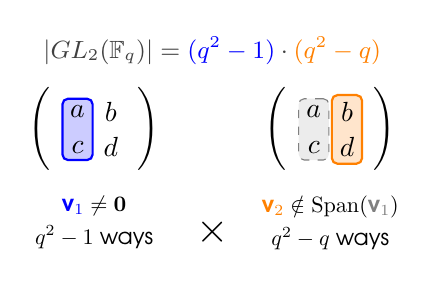
\begin{tikzpicture}[
		font=\sffamily,
		% Style for the matrices
		mtx/.style={
			matrix of math nodes,
			left delimiter=(, right delimiter=),
			nodes={minimum width=1em, inner sep=2pt, anchor=center},
			column sep=2pt, row sep=2pt,
			ampersand replacement=\&
		},
		% Highlighting styles for active columns
		hl-v1/.style={fill=blue!20, draw=blue, thick, rounded corners=2pt, inner sep=.25pt},
		hl-v2/.style={fill=orange!20, draw=orange, thick, rounded corners=2pt, inner sep=.25pt},
		hl-v3/.style={fill=green!20, draw=green!60!black, thick, rounded corners=2pt, inner sep=.25pt},
		hl-v4/.style={fill=purple!20, draw=purple, thick, rounded corners=2pt, inner sep=.25pt},
		% Style for the accumulating "Span Box"
		hl-span/.style={fill=gray!15, draw=gray, dashed, rounded corners=2pt, inner sep=.25pt},
		% Title & Text
		mainTitle/.style={font=\sffamily\bfseries\LARGE, color=darkgray, align=center},
		term label/.style={font=\bfseries\small, align=center}
		]
		
		% CASE m = 2
		\begin{scope}[shift={(1, 4.5)}, scale=1]
			\node[term label, text=darkgray] at (0, 1) {$|GL_2(\mathbb F_q)| = \textcolor{blue}{(q^2-1)} \cdot \textcolor{orange}{(q^2-q)}$};
			\matrix[mtx] (M2_1) at (-1.5, 0) {
					a \& b \\
					c \& d \\
			};
			\begin{scope}[on background layer]
				\node[hl-v1, fit=(M2_1-1-1)(M2_1-2-1)] {};
			\end{scope}
			\matrix[mtx] (M2_2) at (1.5, 0) {
					a \& b \\
					c \& d \\
			};
			\begin{scope}[on background layer]
			\node[hl-span, fit=(M2_2-1-1)(M2_2-2-1)] {}; % v1 is forbidden
			\end{scope}	
			\begin{scope}[on background layer]
				\node[hl-v2, fit=(M2_2-1-2)(M2_2-2-2)] {};
			\end{scope}
			
			\node[below=0.2cm of M2_1, align=center, scale=0.8] {
					$\textcolor{blue}{\textbf{v}_1} \neq \mathbf{0}$ \\[1mm]
					\textbf{$q^2 - 1$} ways
				};
			\node[below=0.2cm of M2_2, align=center, scale=0.8] {
					$\textcolor{orange}{\textbf{v}_2} \notin \mathrm{Span}(\textcolor{gray}{\textbf{v}_1})$ \\[1mm]
					\textbf{$q^2 - q$} ways
				};
			
			% Draw multiplication sign after both nodes exist
			\node[scale=1.5] at ($(M2_1)!0.5!(M2_2)+(0,-1.3)$) {$\times$};
		\end{scope}
	\end{tikzpicture}
\end{document}